\chapter{Конструкторский раздел}

В данном разделе представлены схемы реализуемых алгоритмов и их модификации.

\section{Трудоемкость алгоритмов}\label{estimate}
Для получения функции трудоемкости алгоритма необходимо ввести модель оценки трудоемкости. Трудоемкость "элементарных" операций оценивается следующим образом:
\begin{enumerate}
	\item Трудоемкость 1 имеют операции:
	\begin{equation*}\label{math:simple}
		\begin{array}{cc}
			+, -, =, <, >, <=, >=, ==, +=, -=,\\
			++, --, [], \&\&, ||, >>, << \\
		\end{array}
	\end{equation*}
	\item Трудоемкость 2 имеют операции:
	\begin{equation*}\label{math:complex}
		*, /, \char`\\ , \%
	\end{equation*}	
	\item Трудоемкость конструкции ветвления определяется согласно формуле \ref{math:if}
	\begin{equation}\label{math:if}
		f_{if} = f_{condition} + 
		\begin{sqcases}
			min\left(f_{true} , f_{false}\right) \text{ в лучшем случае,} \\
			max\left(f_{true} , f_{false}\right) \text{ в худшем случае.} \\
		\end{sqcases}
	\end{equation}
	\item Трудоемкость цикла расчитывается по формуле \ref{math:loop}
	\begin{equation}\label{math:loop}
		f_{loop} = f_{init} + f_{cmp} + N \left(f_{body} + f_{inc} + f_{cmp}\right),
	\end{equation}
	\begin{equation*}
		\begin{array}{lllll}
			\text{где} \\
			f_{init} - \text{трудоемкость инициализации,} \\
			f_{body} - \text{трудоемкость тела цикла,} \\
			f_{iter} - \text{трудоемкость инкремента,} \\
			f_{cmp} - \text{трудоемкость сравнения,} \\
			N - \text{количество повторов.}
		\end{array}
	\end{equation*}
	\item Трудоемкость вызова функции равна 0.
\end{enumerate}

\section{Оптимизация алгоритма Копперсмита -- Винограда}\label{sect:optimize}
Алгоритм Копперсмита -- Винограда можно оптимизировать следующим образом:
\begin{itemize}
	\item Счетчики цикла можно объявить единожды и обнулять их по требованию. В этом случае стоимость инициализации при расчете трудоемкости цикла сократится;
	\item Увеличение числа на определенное число можно заменить на операцию $+=$, поскольку она имеет меньший вес чем в сумме сложение и присвоение;
	\item Для алгоритма худшим случаем являются матрицы с нечётным общим размером, а лучшим - с четным. Соответственно, алгоритм можно ускорить в соответствии с четностью размера.
\end{itemize}

\section{Трудоемкость алгоритмов}

\subsection{Классический алгоритм}

Пусть на вход алгоритму поступают матрицы $M_{left}$ и $M_{right}$ с размерностью $n \times m$ и $m \times q$. Тогда трудоемкость классического алгоритма определяется по формуле \ref{math:alg}
\begin{multline}\label{math:alg}
	f_{alg} = f_{loop_i} = 2 + n\left(2 + f_{loop_j}\right) = 2 + n\left(2 + 2 + q\left(2 + f_{loop_k}\right)\right) = \\
	= 2 + n\left(2 + 2 + q\left(2 + +2 + 14 \cdot m\right)\right) \approx 14mnq = 14MNK
\end{multline}
\subsection{Алгоритм Копперсмита — Винограда}

Трудоёмкость алгоритма Копперсмита — Винограда состоит из:
\begin{itemize}
	\item создания и инициализации массивов MH и MV, трудоёмкость которого (\ref{for:init}):
	\begin{equation}
		\label{for:init}
		f_{init} = M + N;
	\end{equation}
	
	\item заполнения массива MH, трудоёмкость которого (\ref{for:MH}):
	\begin{equation}
		\label{for:MH}
		f_{MH} = 2 + K (2 + \frac{M}{2} \cdot 11);
	\end{equation}
	
	\item заполнения массива MV, трудоёмкость которого (\ref{for:MV}):
	\begin{equation}
		\label{for:MV}
		f_{MV} = 2 + K (2 + \frac{N}{2} \cdot 11);
	\end{equation}
	
	\item цикла заполнения для чётных размеров, трудоёмкость которого (\ref{for:cycle}):
	\begin{equation}
		\label{for:cycle}
		f_{cycle} = 2 + M \cdot (4 + N \cdot (11 + \frac{K}{2} \cdot 23));
	\end{equation}
	
	\item цикла, для дополнения умножения суммой последних нечётных строки и столбца, если общий размер нечётный, трудоемкость которого (\ref{for:last}):
	\begin{equation}
		\label{for:last}
		f_{last} = \begin{cases}
			2, & \text{чётная,}\\
			4 + M \cdot (4 + 14N), & \text{иначе.}
		\end{cases}
	\end{equation}
\end{itemize}

Итого, для худшего случая (нечётный общий размер матриц) имеем (\ref{for:bad}):
\begin{equation}
	\label{for:bad}
	f =  f_{MH} + f_{MV} + f_{cycle} + f_{last}\approx 11.5 \cdot MNK
\end{equation}

Для лучшего случая (чётный общий размер матриц) имеем (\ref{for:good}):
\begin{equation}
	\label{for:good}
	f =  f_{MH} + f_{MV} + f_{cycle} + f_{last} \approx 11.5 \cdot MNK
\end{equation}


\subsection{Оптимизированный алгоритм Копперсмита — Винограда}

Оптимизированный алгоритм Винограда представляет собой обычный алгоритм Винограда, за исключением следующих оптимизаций:
\begin{itemize}
	\item вычисление происходит заранее;
	\item используется битовый сдвиг, вместо деления на 2;
	\item последний цикл для нечётных элементов включён в основной цикл,
	используя дополнительные операции в случае нечётности N.
\end{itemize}


Трудоёмкость улучшенного алгоритма Копперсмита — Винограда состоит из:
\begin{itemize}
	\item создания и инициализации массивов MH и MV, трудоёмкость которого (\ref{for:impr_init}):
	\begin{equation}
		\label{for:impr_init}
		f_{init} = M + N;
	\end{equation}
	
	\item заполнения массива MH, трудоёмкость которого (\ref{for:impr_MH}):
	\begin{equation}
		\label{for:impr_MH}
		f_{MH} =  2 + K (2 + \frac{M}{2} \cdot 8);
	\end{equation}
	
	\item заполнения массива MV, трудоёмкость которого (\ref{for:impr_MV}):
	\begin{equation}
		\label{for:impr_MV}
		f_{MV} =  2 + K (2 + \frac{M}{2} \cdot 8);
	\end{equation}
	
	\item цикла заполнения для чётных размеров, трудоёмкость которого (\ref{for:impr_cycle}):
	\begin{equation}
		\label{for:impr_cycle}
		f_{cycle} =2 + M \cdot (4 + N \cdot (11 + \frac{K}{2} \cdot 18));
	\end{equation}
	
	\item условие, для дополнения умножения суммой последних нечётных строки и столбца, если общий размер нечётный, трудоемкость которого (\ref{for:impr_last}):
	\begin{equation}
		\label{for:impr_last}
		f_{last} = 
		\begin{cases}
			1, & \text{чётная,}\\
			4 + M \cdot (4 + 10N), & \text{иначе.}
		\end{cases}
	\end{equation}
\end{itemize}

Итого, для худшего случая (нечётный общий размер матриц) имеем (\ref{for:bad_impr}):
\begin{equation}
	\label{for:bad_impr}
	f = f_{MH} + f_{MV} + f_{cycle} + f_{last} \approx 9MNK
\end{equation}

Для лучшего случая (чётный общий размер матриц) имеем (\ref{for:good_impr}):
\begin{equation}
	\label{for:good_impr}
	f = f_{MH} + f_{MV} + f_{cycle} + f_{last} \approx 9MNK
\end{equation}

\section{Схемы алгоритмов}
На рисунке \ref{fig:alg} приведена схема классического алгоритма умножения матриц. На рисунке \ref{fig:win-1} приведена схема алгоритма Копперсмита -- Винограда. Рисунок  
\ref{fig:win-2} демонстрируют схему оптимизированного алгоритма Копперсмита -- Винограда.\newpage

\begin{figure}[ht!]
	\centering
	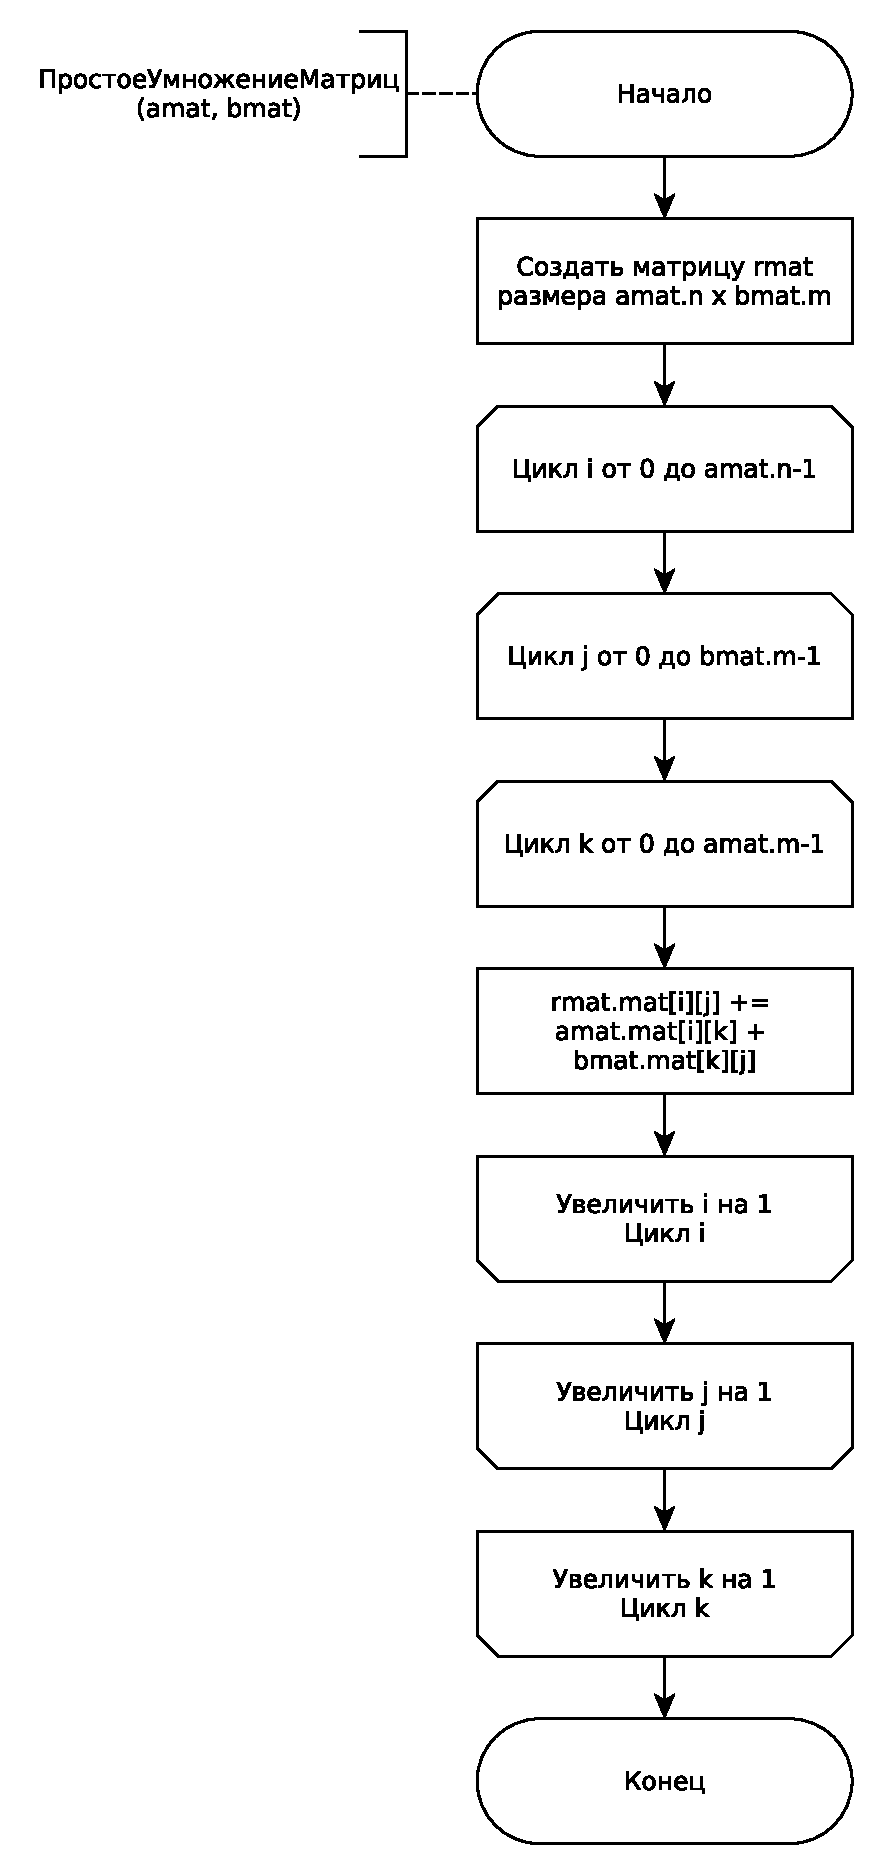
\includegraphics[width=0.65\linewidth]{assets/mtx-alg.pdf}
	\caption{Схема классического алгоритма умножения матриц}
	\label{fig:alg}
\end{figure}

\begin{figure}[ht!]
	\centering
	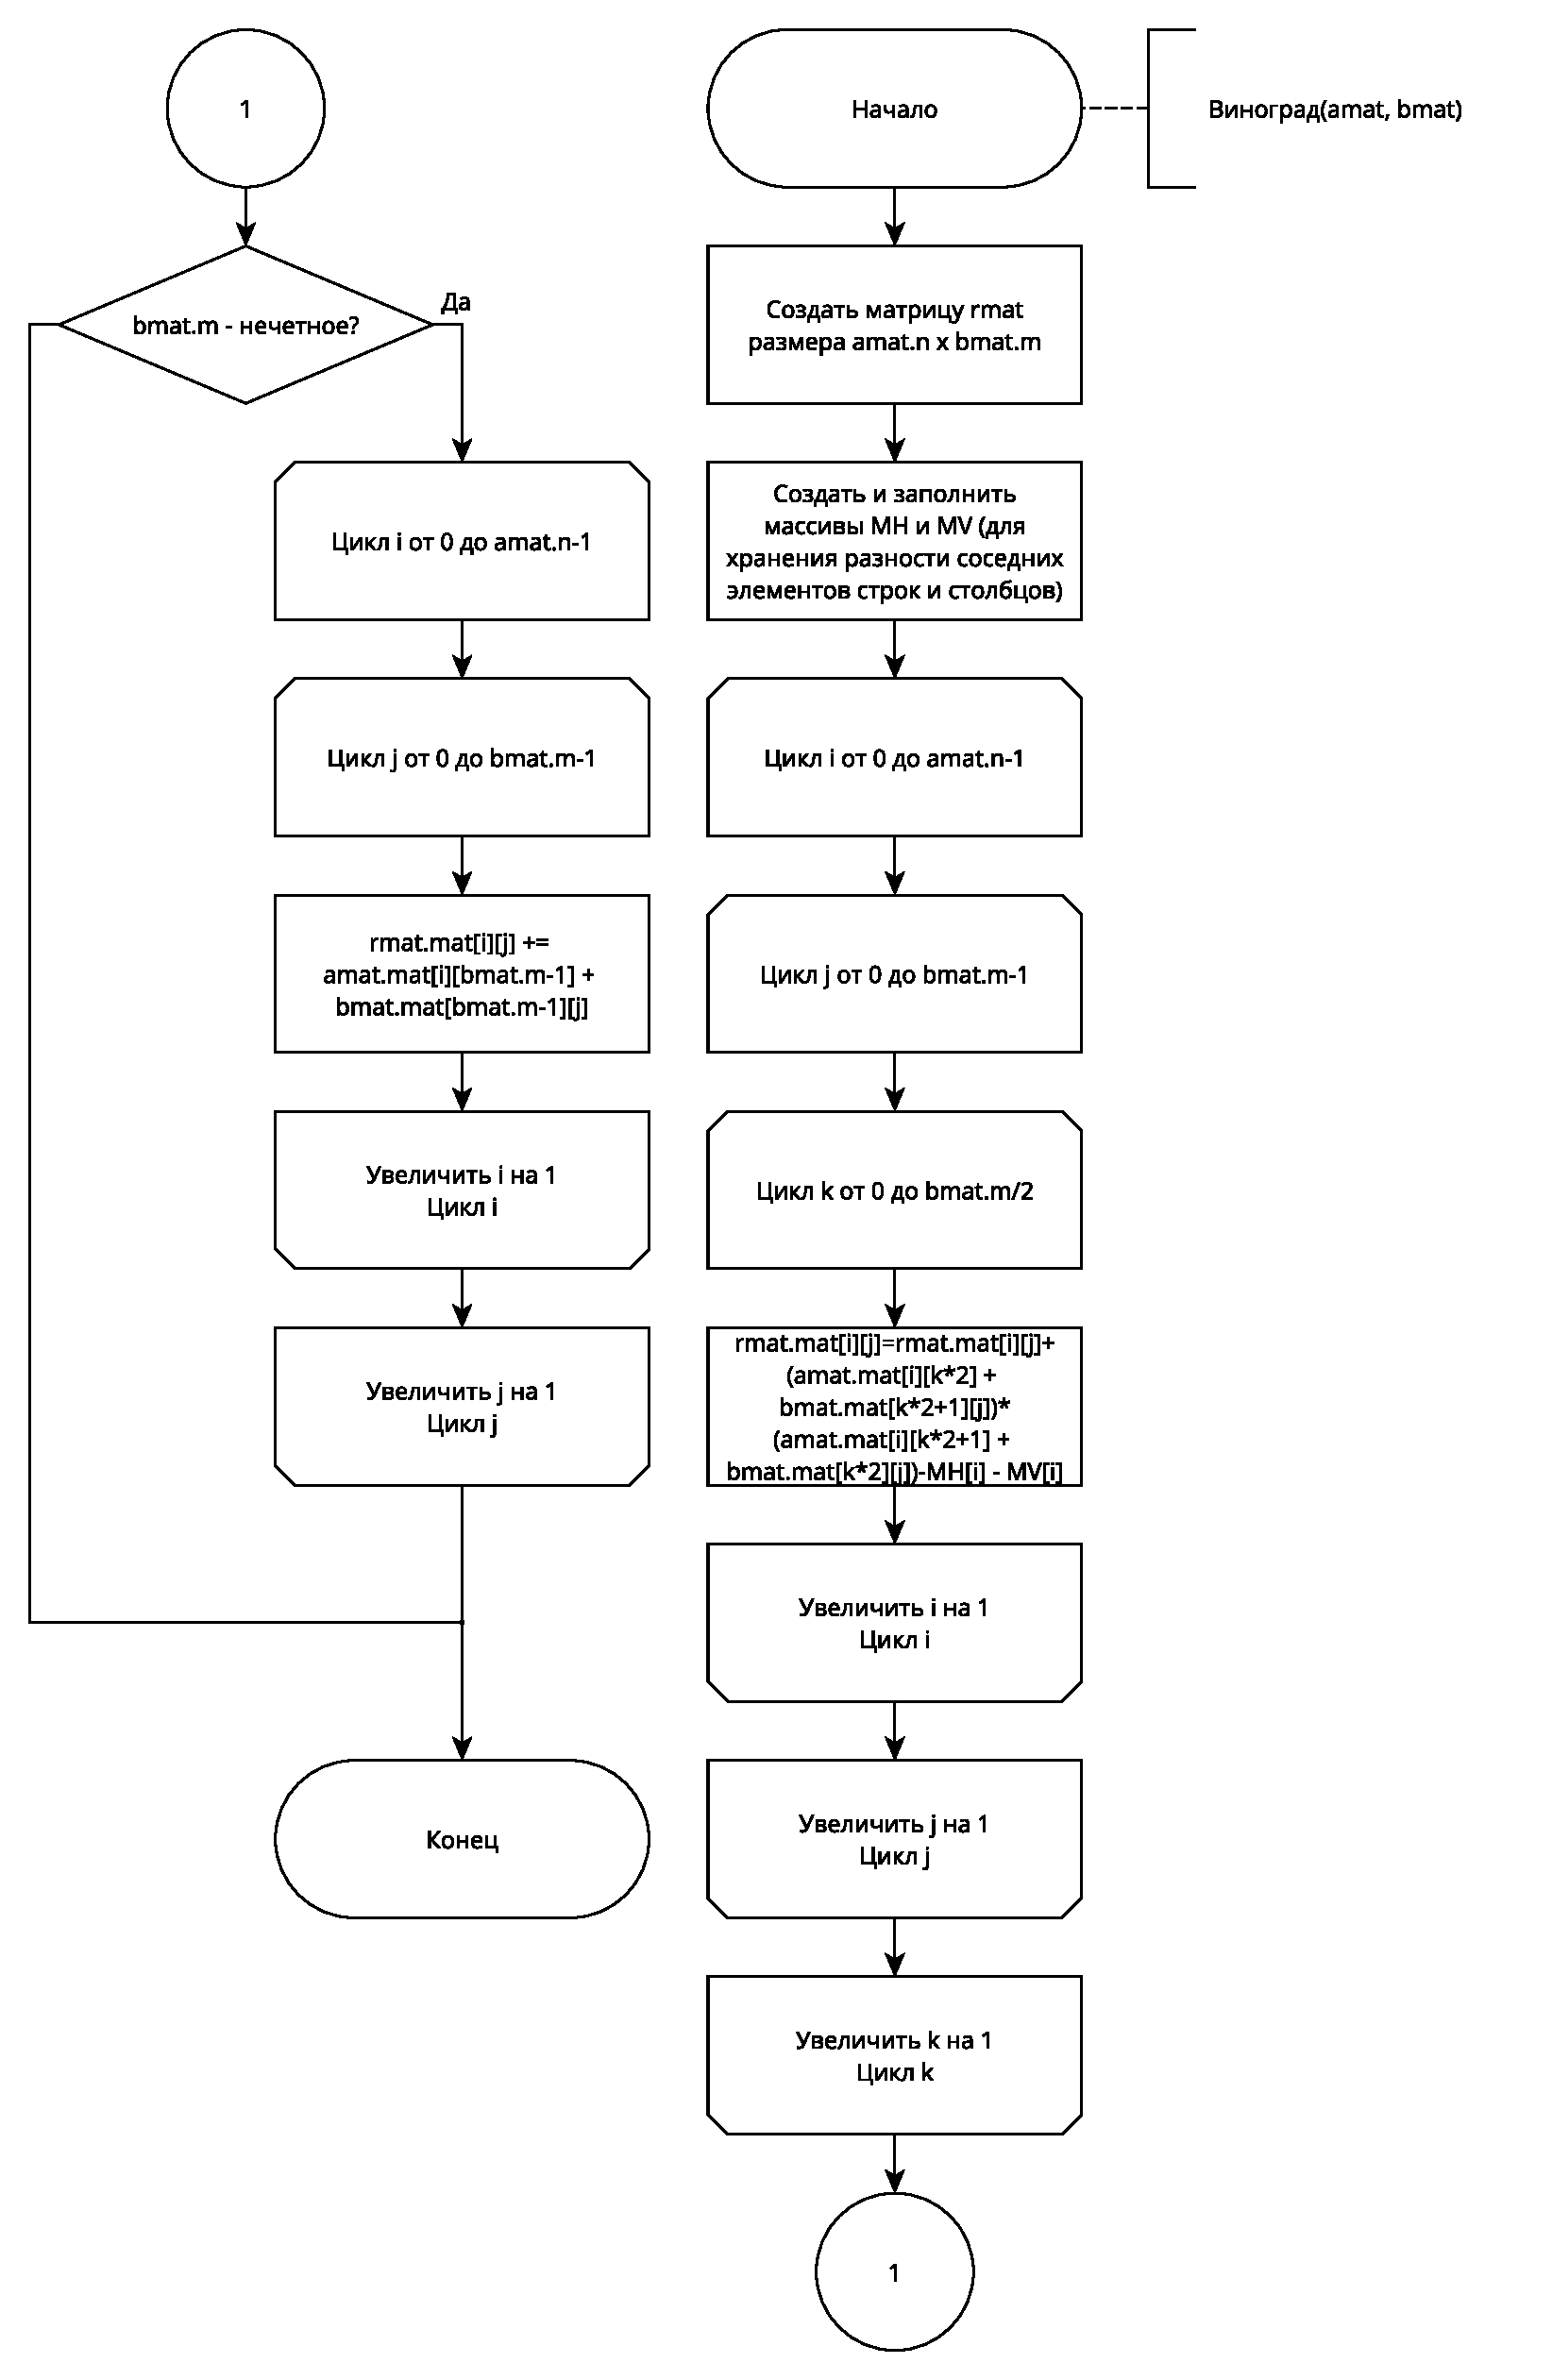
\includegraphics[width=0.95\linewidth]{assets/mtx-win1.pdf}
	\caption{Схема алгоритма умножения матриц Копперсмита -- Винограда}
	\label{fig:win-1}
\end{figure}

\begin{figure}[ht!]
	\centering
	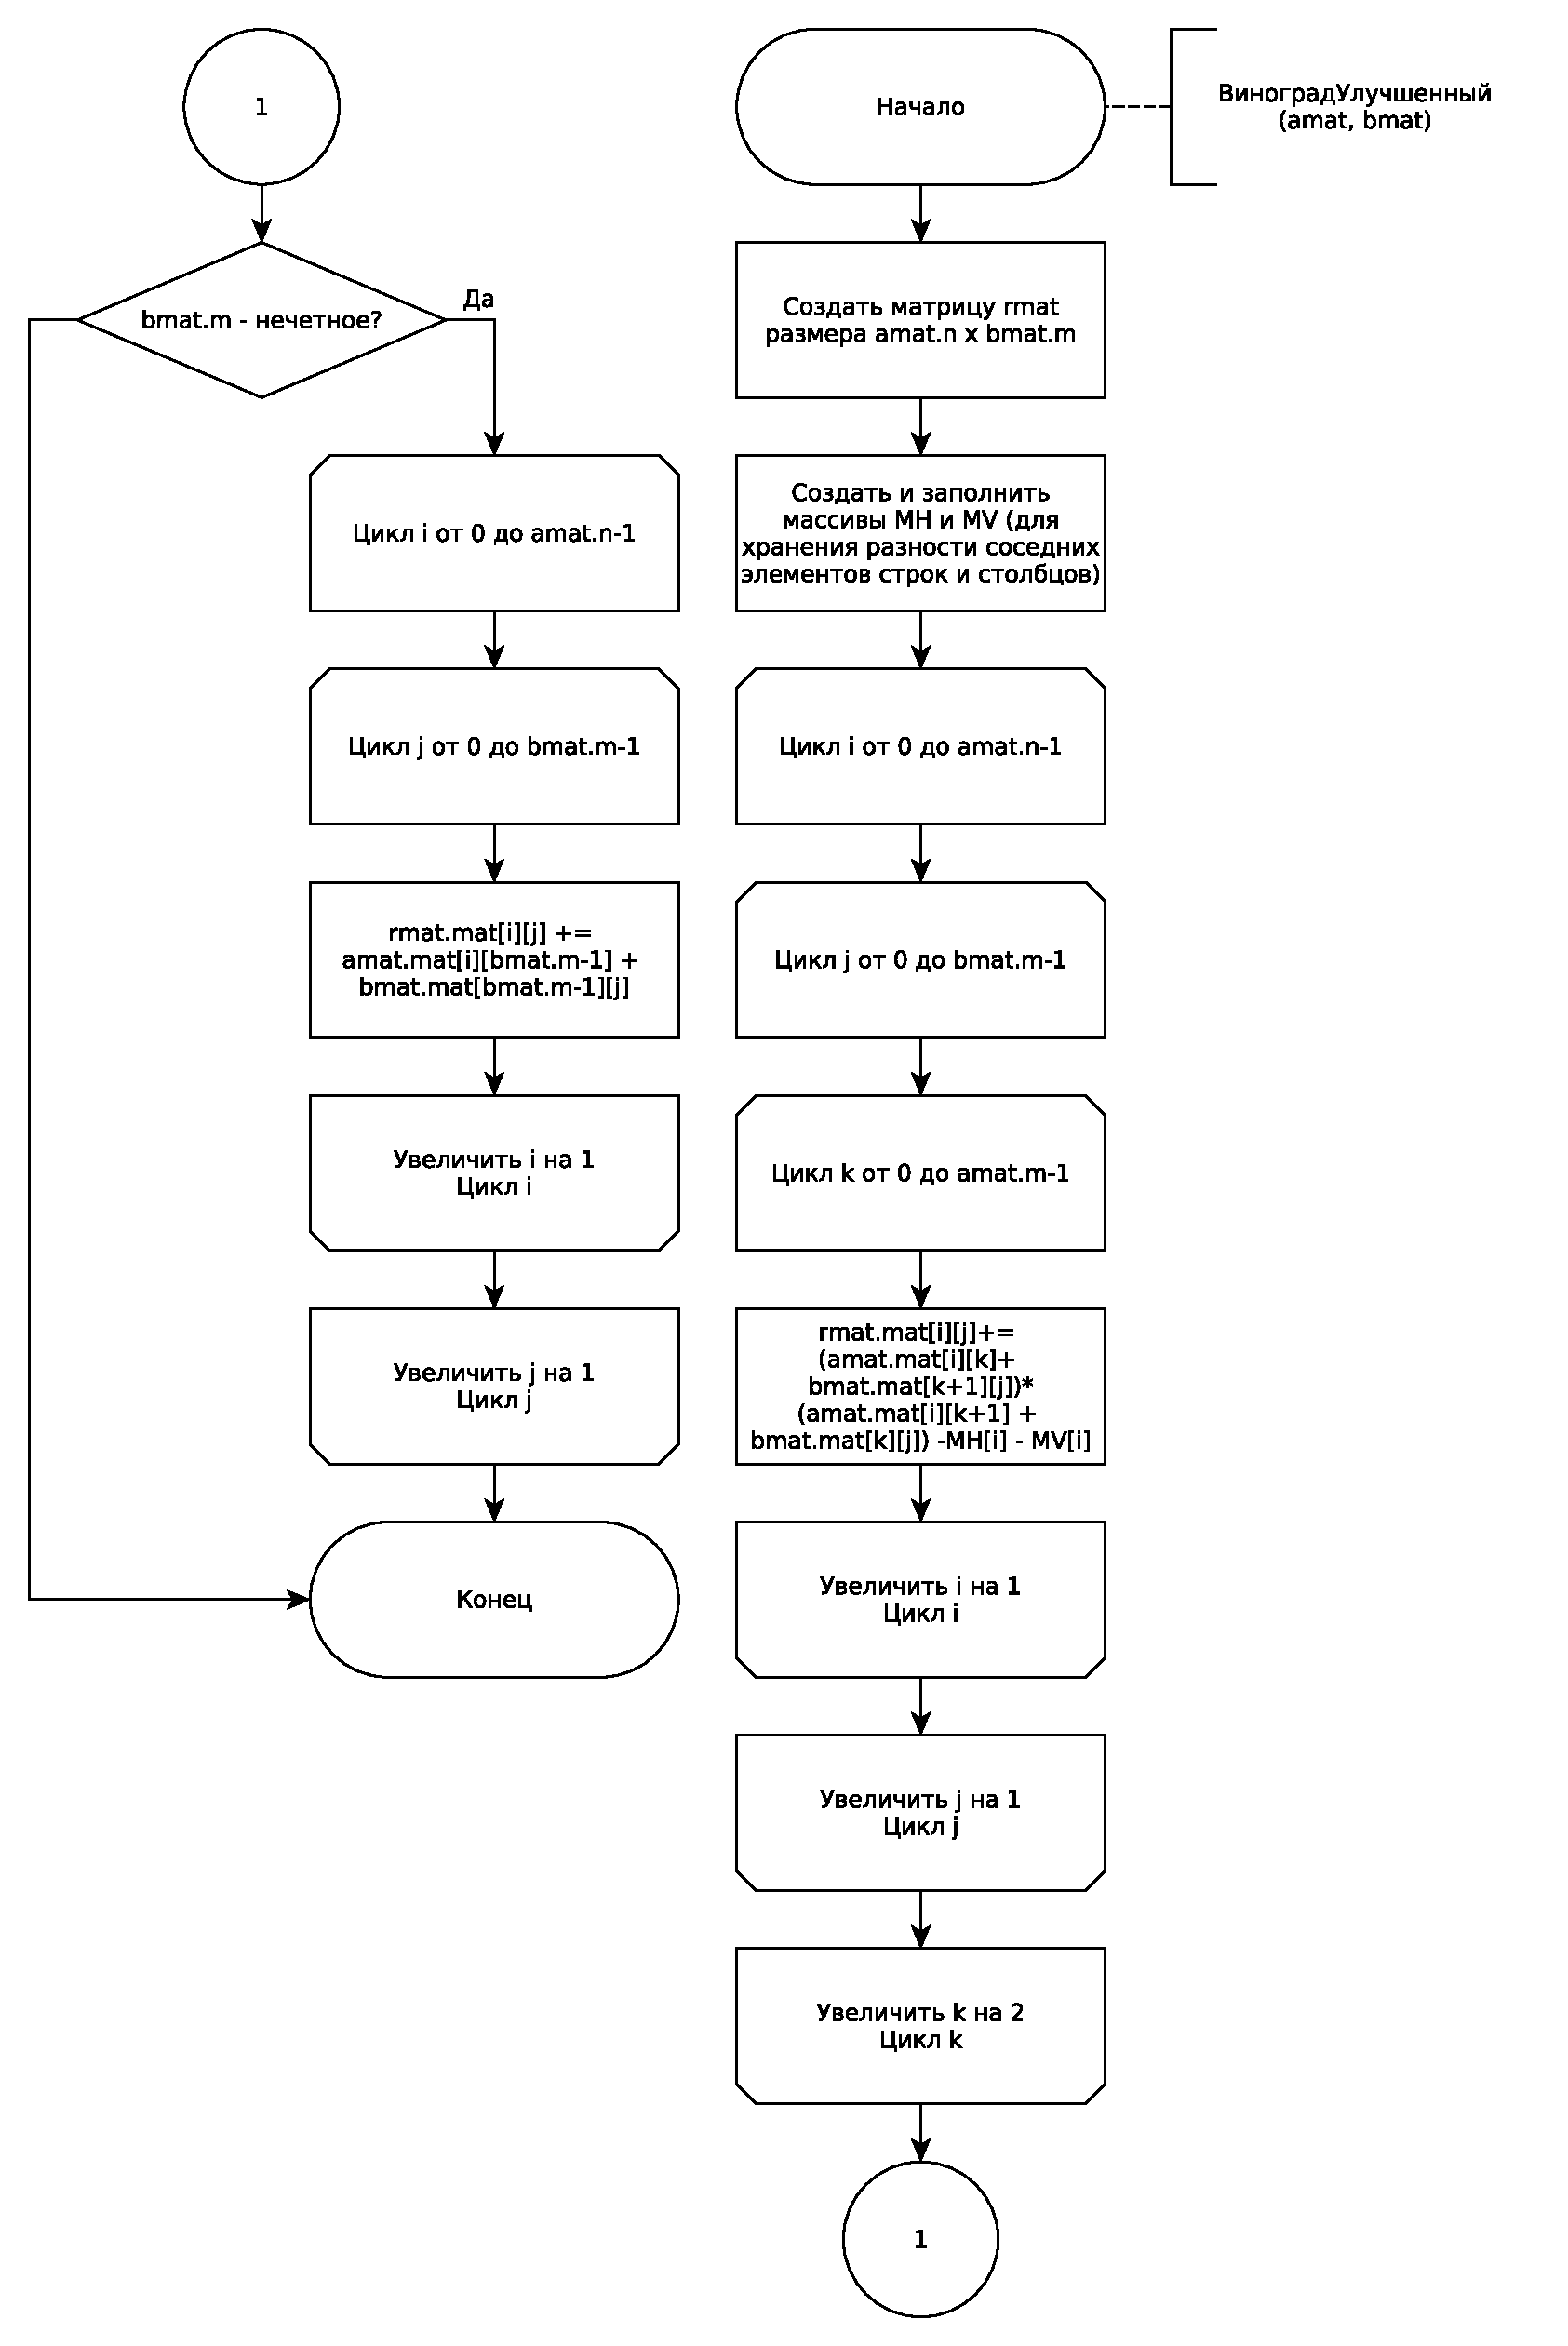
\includegraphics[width=0.95\linewidth]{assets/mtx-win2.pdf}
	\caption{Схема оптимизированного алгоритма умножения матриц Копперсмита -- Винограда}
	\label{fig:win-2}
\end{figure}


\subsection{Вывод}
Алгоритмы были проанализированы с точки зрения временных затрат. Было выявлено, что алгоритм Копперсмита -- Винограда работает на \\ $1.5MNK$ быстрее, чем классический матричный. Оптимизация алгоритма же дает выигрыш на $2.5MNK$. 


Были построены схемы алгоритмов. Теоретически были исследованы способы оптимизации алгоритма Копперсмита -- Винограда. Было получено достаточно теоретических сведений для разработки ПО, решающего поставленную задачу.